\begin{figure}
	\centering
	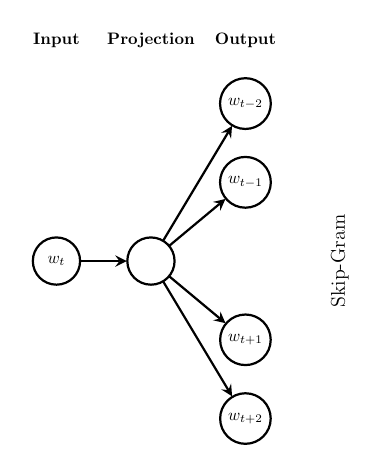
\begin{tikzpicture}[
		scale=0.4,
		every node/.style={scale=0.6},
		n/.style={circle,draw=black,thick,minimum width=1cm},
		arr/.style={-stealth,thick}
	]

		\node[rotate=90] at (6,0) {\highlight{\large Skip-Gram}};
		
		% input
		\node at (-3,7) {\textbf{Input}};
		\node[n] (I1) at (-3,0) {$\bm{w}_t$};
	

		% projection
		\node at (0,7) {\textbf{Projection}};
		\node[n] (P1) at (0,0) {};

		% output
		\node at (3,7) {\textbf{Output}};
		\node[n] (O1) at (3,5) {$\bm{w}_{t-2}$}; 
		\node[n] (O2) at (3,2.5) {$\bm{w}_{t-1}$};
		\node[n] (O3) at (3,-2.5) {$\bm{w}_{t+1}$}; 
		\node[n] (O4) at (3,-5) {$\bm{w}_{t+2}$};
		
		% connections
		\draw[arr] (I1) -- (P1);
		\draw[arr] (P1) -- (O1); \draw[arr] (P1) -- (O2); \draw[arr] (P1) -- (O3); \draw[arr] (P1) -- (O4);

	\end{tikzpicture}
\end{figure}